\begin{problem}{Maurar}{Inn}{Út}{~}{~}

	Her af maurum gengur á láréttri stöng af lengd $l$ cm, hver með fasta hraðan $1$ cm/s. Þegar maur kemur að öðrum hvorum enda stangarinnar, þá dettur hann um leið af stönginni. Þegar tveir maurar mæta hvorum öðrum, þá snúa þeir báðir við og byrja að ganga í burtu frá hvorum öðrum. Við vitum upphafsstöðu hvers maurs á stönginni, en við vitum því miður ekki í hvaða átt hver maur er að ganga. Á endanum munu allir maurarnir detta af stönginni. Þitt verkefni er að reikna bæði út fyrsta mögulega tímann, og síðasta mögulega tímann á að allir maurarnir detta af stönginni.

	\begin{figure}[h]
		\centering
		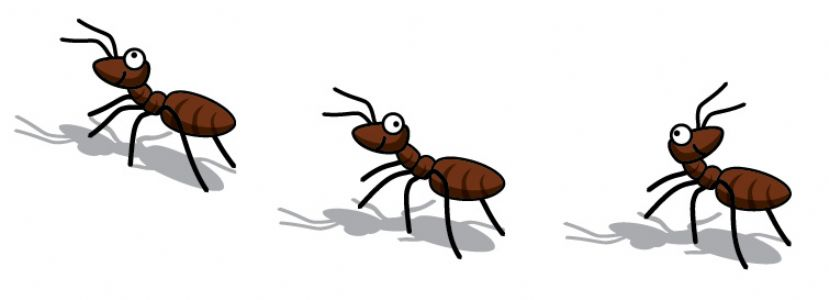
\includegraphics[scale=0.3]{../Maurar/ants.jpg}
	\end{figure}

	\Input

		Á fyrstu línu er heiltalan $1 \leq T \leq 100$, sem táknar fjölda prófunartilvika sem fylgja. Hvert prófunartilvik samanstendur af tveimur línum.

		Fyrri línan inniheldur tvær heiltölur $0 \leq l \leq 10000$ og $1 \leq n \leq 1000$, þar sem $l$ táknar lengd stangarinnar (í cm) og $n$ táknar fjölda maura á stönginni.

		Seinni línan inniheldur $n$ heiltölur, aðskildar með bili, sem tákna upphafsstöðu hvers maurs mælda frá vinstri enda stangarinnar. Upphafsstöðurnar eru ekki í neinni sérstakri röð, en gera má ráð fyrir að engir tveir maurar byrji á sama stað.

	\Output

		Fyrir hvert prófunartilvik á að skrifa út eina línu sem inniheldur tvær heiltölur. Fyrri heiltalan táknar fyrsta mögulega tímann á því að allir maurar detta af stönginni (ef upphaflegu áttir hvers maurs eru valdar á viðeigandi hátt), en seinni heiltalan táknar síðasta mögulega tímann á að það gerist.

	\Examples

\begin{example}
\exmp{%
2
10 3
2 6 7
214 7
11 12 7 13 176 23 191
}{%
4 8
38 207
}%
\end{example}
\end{problem}